\documentclass[12pt,openright,twoside]{book}
\usepackage{graphicx}
\usepackage{geometry}
\usepackage{pdflscape}
\usepackage{natbib}
\usepackage{amsmath}
\usepackage{pdflscape}
%%\usepackage{tabu}
\usepackage{caption}
%%\usepackage{floatrow}
\usepackage{enumerate}
\usepackage{enumitem}
\usepackage{titlesec}
\usepackage{wrapfig}
\usepackage{bm}
\usepackage{booktabs} % For \toprule, \midrule and \bottomrule
\usepackage{siunitx} % Formats the units and values
\usepackage{pgfplotstable} % Generates table from .csv
\usepackage{physics}
\usepackage{url}
\usepackage{float}
\usepackage{listings}


\titleformat{\chapter}
  {\Large\bfseries} % format
  {}                % label
  {0pt}             % sep
  {\LARGE}           % before-code
\renewcommand{\figurename}{\textbf{Figure}}
\renewcommand{\tablename}{\textbf{Table}}
\newcommand{\HRule}{\rule{\linewidth}{0.4mm}}

\renewcommand{\contentsname}{{\Huge Table of contents}}
\renewcommand{\chaptername}{{\Huge  }}
%\renewcommand{\thebibliography}{\Bibliografie}


\geometry{
 a4paper,
 total={210mm,297mm},
 left=25.0mm,
 right=25.0mm,
 top=25.0mm,
 bottom=30.0mm,
 }

 \setcounter{tocdepth}{3}
%level -1: part, 0: chapter, 1: section, etc.

\sisetup{
  round-mode          = places, % Rounds numbers
  round-precision     = 2, % to 2 places
}

\begin{document}

\begin{titlepage}
\begin{center}






\includegraphics[width=16cm]{./antet_L.jpg}



\vspace{4cm}



    \HRule \\[0.3cm]


    {\Large \textsc {Numerical integration of highly oscillating functions}}\\


  \HRule \\[1.1cm]

  \textsc{\large Bachelor Thesis}\\[4cm]

   \begin{flushleft} \large
    {Author} \\[0.1cm]
    Radu-Mihai T\^{i}rc\u{a}
   \end{flushleft}

   \begin{flushright} \large
    {Scientific coordinator} \\[0.1cm]
    Conf. dr. M\u{a}d\u{a}lina Boca
   \end{flushright}


  \vfill

  % Partea de jos a paginii
 %% {\large \today}

 {\large Bucure\c{s}ti, 2020}

\end{center}

\end{titlepage}

\newpage
\vspace*{\fill}
\thispagestyle{empty}




\newpage
\thispagestyle{plain} \pagenumbering{roman}


\vspace*{36pt}

\begin{center}

{\LARGE \textbf{Acknowledgements}}

\end{center}

\vspace{36pt}
Foremost I would like to express my sincere gratitude to my scientific coordinator and advisor Conf.dr. M\v ad\v alina Boca for the continuous support provided for the development of my Bachelor's Thesis and for her patience, motivation and insight. Her guidance helped me throughout the process of writing my thesis. \\

I would also like to thank Virgil Baran for his help with the implementation of the code that this thesis is based upon. His insight was very valuable to my process.
\vspace{40pt}


%%\noindent\textbf{NB} \textit{Mul\c{t}umiriile pot fi incluse aici, nu este necesar un capitol special }

\vspace*{\fill}
\newpage
\thispagestyle{empty} \vspace*{\fill} \tableofcontents

\setlength\parindent{0pt}



\setcounter{page}{0}

%% this comand remove indent

\newpage

 \pagenumbering{arabic}
\chapter{Introducere}

\paragraph{} In this paper, we will showcase different methods of numerical integration for highly oscillating functions. These types of functions are particularly difficult to compute because, due to their steep oscillatory nature, they cannot be properly approximated using traditional methods.

We approach this challenging topic making use of the Filon quadrature, named so for, which is a more than appropriate method for rapidly oscillating functions such as
\begin{figure}[h]
    \centering
    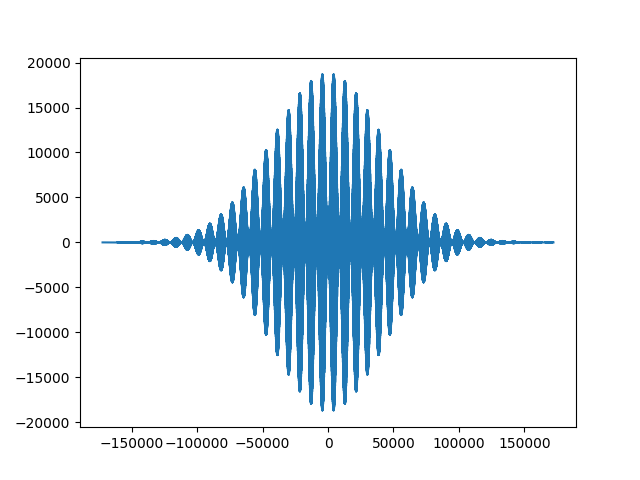
\includegraphics[scale=0.7]{c1/Figure_1.png}
    \caption{An example function}
    \label{fig:my_label}
\end{figure}

These type of "unusual" functions can be found, perhaps unsurprisingly, in a wide array of applications such as laser and radiation applications \cite{book1}, electrical engineering \cite{circ} \cite{circ2}, Quantum Field theory \cite{world}, far-field theory in aerodynamics\cite{aer} and, of course, mathematics\cite{rules} \cite{fcc} \cite{comp}. 

The pervasiveness of highly oscillating integrals that need solving definitely raises our interest in the Filon quadrature since it is a relatively straightforward and simple method that is taylor-made exactly for this type of difficult integrals.%%%Local Variables:
%%% mode: latex
%%% TeX-master: "../th"
%%% End:

% !TeX root = ../diss.tex
\chapter{Metoda Filon}
\label{cap:cap2}

\section{Numerical integration}
%Rectangle rule

\paragraph{} Numerical integration is comprised of a broad family of algorithms that aim to numerically compute values of finite integrals.
All can be traced back to this simplest form:

\begin{equation}
    \int_a^b f(x) dx \approx (b-a) f\left(\frac{a+b}{2}\right),\label{rectangle}
\end{equation}

which is known as "rectangle rule". This is the procedure trough which the area underneath a function, up to the $"x"$ axis, is approximated with a rectangle. This gives a very rough approximate of the actual integral


%Trapezoidal rule

A better approximation is given by this formula: 

\begin{equation}
    \int_a^b f(x) dx \approx (b-a) \left(\frac{f(a)+f(b)}{2}\right),\label{trapezoid}
\end{equation}

which approximates the area with a trapezoid, thus giving it the name "trapezoidal rule".

%Composite Trapezoidal rule

For both of these methods, the accuracy of the result can be virtually infinitely improved by dividing the $[a,b]$ interval in finer and finer $n$ subintervals.
This, in the case of the "trapezoidal rule" yields the following formula:

\begin{equation}
    \int_a^b f(x) dx \approx \frac{b-a}{n}\left(\frac{f(a)}{2}+\sum_{k=1}^{n-1}\left(f\left(a+k\frac{b-a}{n}\right)\right)+\frac{f(b)}{2}\right),\label{composite}
\end{equation}
where the sub intervals are of the form $ [a+kh,a+(k+1)h] \subset [a,b], h=\frac{b-a}{n} $.

These methods are generally referred to as "quadratures". The therm, "quadrature", has been historically used to describe the process of determining area. Now, it is somewhat loosely used to describe pretty much all numerical integration methods.

\section{Quadrature}

\paragraph{} Quadrature rules can be derived by constructing interpolating functions that are easy to integrate numerically.
The interpolating function can be a polynomial of degree zero (a constant function) like in the case of the rectangle rule\eqref{rectangle},
where the interpolation point is $\left(\frac{a+b}{2},f\left(\frac{a+b}{2}\right)\right)$. Similarly, for the trapezoidal rule\eqref{trapezoid}, the interpolating function is a polynomial of degree 1 (a straight line) that passes through two points $(a,f(a))$ and $(b,f(b))$. 
In the case of the composite rule\eqref{composite}, the number of interpolation points is directly proportional with the number of subintervals or steps, $n$. Interpolation with polynomials evaluated at equally spaced points yields a Newton-Cotes formula of which the previously mentioned methods ar a type.

\paragraph{} We have the general quadrature formula: 


\begin{equation}
    \int_a^b dx f(x)  \approx \sum_{i=1}^n w_if(x_i), \quad a \leq x_i \leq b,\label{quadrature}
\end{equation}
    
%\paragraph{Gausian quadrature}is the most common type of numerical quadrature. It is suitable to yield exact values for polynomials of degree $2n-1$,
%but can also offer 

%To be completed

\section{Oscillatory integrals with constant oscillation frequency}


The types of integrals that we address are of the form:

\begin{equation}
    I[a,b] = \int_a^b dx \varphi(x)e^{i\omega x}\label{oscillatoryIntegral}
\end{equation}

\paragraph{}Here we find $\varphi(x)$, the preexponential and our oscillatory component $e^{i\omega x}$ with the constant oscillation frequency $\omega$.
Under the assumption that $\varphi(x)$ is slowly oscillating, Filon suggests dividing the integration interval in $N$ subintervals and apply a 3-point quadrature scheme on each of these, where only the preexponential function $\varphi(x)$ is interpolated as opposed to the whole integrand.
Afterwards, the entire integral is approximated at $2n+1$ nodes. 

\paragraph{}Each subinterval is interpolated by a 3-point scheme:

\begin{equation}
    I(x_n,x_{n+2}) = \int_{x_n}^{x_{n+2}} dx \varphi(x)e^{i\omega x} \approx w_n\varphi_n+w_{n+1}\varphi_{n+1}+w_{n+2}\varphi_{n+2}\label{subintervalInterpolation}
\end{equation}

Where $\varphi(x)$ is approximated by a second degree polynomial, 

\begin{equation}
    \varphi(x) \approx c_0 + c_1x + c_2x^2\label{IntegrandAproximation}
\end{equation}

It is important to note that if this approximation is exact, the equation\eqref{subintervalInterpolation} gives an exact value for $I(x_n,x_{n+2})$.

The next step is to find the weights $w_n$. This is achieved by integrating over the three moments: 

\begin{equation}
    J_{l}=:\int_{x_{n}}^{x_{n+2}} x^{l} \mathrm{e}^{\mathrm{i} \omega x}=w_{n} x_{n}^{l}+w_{n+1} x_{n+1}^{l}+w_{n+2} x_{n+2}^{l} \quad l \in\{0,1,2\}
\end{equation}

It is an important assumption of the Filon method that the $J_l$ moments can be solved analyticall.  
After solving the system, we find: 

\begin{equation}
    \begin{aligned}
        w_{n+l} &=\zeta_{l} h \mathrm{e}^{\mathrm{i} \omega x_{n+l}} \\
        \zeta_{0} &=\zeta_{a}+\mathrm{i} \zeta_{b} \\
        \zeta_{a} &=\frac{3 \Theta+\cos (2 \Theta) \Theta-2 \sin (2 \Theta)}{2 \Theta^{3}} \\
        \zeta_{b} &=\frac{2 \Theta^{2}+2 \cos (2 \Theta)+\sin (2 \Theta) \Theta-2}{2 \Theta^{3}} \\
        \zeta_{1} &=\frac{4(\sin (\Theta)-\Theta \cos (\Theta))}{\Theta^{3}} \\
        \zeta_{2} &=\zeta_{a}-\mathrm{i} \zeta_{b}
    \end{aligned} \label{moments}
\end{equation}

with the parameter $\Theta$ defined as $\Theta=\omega h$ and $h$ being the step size ($h=\frac{b-a}{N}$).

\paragraph{}Inserting all this in the equation\eqref{subintervalInterpolation} and some further processing we find:

\begin{equation}
    \begin{aligned}
        \int_{x_{n}}^{x_{n+2}} d x \varphi(x) \mathrm{e}^{\mathrm{i} \omega x} \approx Q^{\text{F}}(x_n,x_{n+2})=
        & h\left[\mathrm{i} \alpha\left(\varphi_{n} \mathrm{e}^{\mathrm{i} \omega x_{n}}-\varphi_{n+2} \mathrm{e}^{\mathrm{i} \omega x_{n+2}}\right)\right.\\
        &+\beta \left(\varphi_{n} \mathrm{e}^{\mathrm{i} \omega x_{n}}+\varphi_{n+2} \mathrm{e}^{\mathrm{i} \omega x_{n+2}}\right) \\
        &\left.+\gamma \varphi_{n+1} \mathrm{e}^{\mathrm{i} \omega x_{n+1}}\right]
    \end{aligned}
\end{equation}
with $\alpha, \beta, \gamma$ defined as:
\begin{equation}
    \begin{aligned}
        &\alpha=\alpha(\Theta)=\frac{2 \Theta^{2}-2 \sin ^{2}(\Theta)+\sin (2 \Theta) \Theta}{2 \Theta^{3}}\\
        &\beta=\beta(\Theta)=\frac{2 \Theta\left(1+\cos ^{2}(\Theta)\right)-2 \sin (2 \Theta)}{2 \Theta^{3}}\\
        &\gamma=\gamma(\Theta)=\frac{4(-\Theta \cos (\Theta)+\sin (\Theta))}{\Theta^{3}}
    \end{aligned}
\end{equation}

It should be noted that for small $\Theta$, these parameters have the Taylor expansions:

\begin{equation}
    \begin{array}{l}
        \alpha(\theta)=\frac{2}{45} \theta^{3}-\frac{2}{313} \theta^{5}+\frac{2}{4725} \theta^{7}+\cdots \\
        \beta(\theta)=\frac{2}{3}+\frac{2}{15} \theta^{2}-\frac{4}{105} \theta^{4}+\frac{2}{567} \theta^{6}+\cdots \\
        \gamma(\theta)=\frac{4}{3}-\frac{2}{15} \theta^{2}+\frac{1}{210} \theta^{4}-\frac{1}{11340} \theta^{6}+\cdots
        \end{array}.
\end{equation}

The summation of these contributions over all the subintervals, brings us to the textbook formula for the Filon quadrature:

\begin{equation}
    \begin{aligned}
        \int_{a}^{b} d x \varphi(x) \mathrm{e}^{\mathrm{i} \omega x}=& \sum_{n=0}^{N-1} \int_{x_{2 n}}^{x_{2 n+2}} d x \varphi(x) \mathrm{e}^{\mathrm{i} \omega x} \approx \sum_{n=0}^{N-1} Q^{\text {F}}\left(x_{2 n}, x_{2 n+2}\right) \\
        =& h\left[\mathrm{i} \alpha\left(\varphi_{0} \mathrm{e}^{\mathrm{i} \omega x_{0}}-\varphi_{2 N} \mathrm{e}^{\mathrm{i} \omega x_{2 N}}\right)\right.\\
        &+\beta\left(\sum_{n=0}^{N} \varphi_{2 n} \mathrm{e}^{\mathrm{i} \omega x_{2 n}}-\frac{1}{2}\left[\varphi_{2 N} \mathrm{e}^{\mathrm{i} \omega x_{2 N}}+\varphi_{0} \mathrm{e}^{\mathrm{i} \omega x_{0}}\right]\right) \\
        &\left.+\gamma \sum_{n=1}^{N} \varphi_{2 n-1} \mathrm{e}^{\mathrm{i} \omega x_{2 n-1}}\right] \\
        &+\mathcal{O}\left(h^{4}\right)
    \end{aligned}
\end{equation}

%%% Local Variables:
%%% mode: latex
%%% TeX-master: "../th"
%%% End:

\chapter{Filon Method Generalization}

\section{The issue}

\paragraph{} The Filon method in its pure form is only suited for \eqref{oscillatoryIntegral}.
In real-world applications it isn't very often that these type of functions are found. The problem arises with the fact that the $\theta$ \eqref{moments} parameter depends on the oscillation frequency $\omega$, but the parameter needs to be constant.

This means that the oscillation frequency is going to be a function of its own. This function will have to be monotonous such that the solution that is to be provided is going to work. 

\section{Univariate Dynamic Integral}

The now expanded form of the integrals that are to be calculated is:

\begin{equation}
    \int_{a}^{b}dxA(x)e^{ih(x)}
\end{equation}

where $h(x)$ is the new, variable oscillation frequency.

In order to be able to compute this type of integral \cite{book1}, we need to bring it into a Filon compatible form. This means that we have to re-parameterize $h(x)$ onto a variable that rises linearly from its minimal value $h(x_{min})$, up to its maximal value $h(x_{max})$.

\begin{equation}
    h(x)=y \label{parameterization}   
\end{equation}

This is achieved by applying a change of variable:

\begin{equation}
    y=h(x), \quad \dd y=\dv{f}{x} \dd x, \quad \dd x=\frac{\dd y}{\left(\dv{f}{x}\right)} \label{changeOfVariable}
\end{equation}

Having previously imposed the constraint of monotony, it is now clear that the $\dv{f}{x}$ denominator will not vanish.

\begin{equation}
    \int_{y_a}^{y_b}dy\frac{A(x(y))}{\dv{f}{x}\left(x(y)\right)}e^{iy}
\end{equation}


In this new form of the integral, another issue arises from a numerical stand point. 
The Filon method requires an equidistant array of values as integration domain.

\begin{equation}
    x = [x_1, x_2, x_3, ..., x_N]; \quad x_1 = a, x_N = b; \quad step = \Delta x = \frac{b-a}{n}. 
\end{equation}\\

The newly obtained array: 
\begin{equation}
    y_t=h(x)=[h(x_1),h(x_2),h(x_3), ..., h(x_N)]; \quad y_a=h(x_1), y_b=h(x_N) 
\end{equation}

is evidently not an equidistant one, but inherits the monotony of its generator function $h(x)$, such that:
$$
    y_{t1}=h(x_1) < y_{t2}=h(x_2) < y_{t3}=h(x_3) < ... < y_{tN}=h(x_N).
$$

The next step is to find the $x(y)$ array, bound by $y_a$ and $y_b$ such that:

\begin{equation}
        y = [y_1, y_2, y_3, ..., y_N]; \quad y_N-y_{N-1}=\Delta y = \frac{y_b-y_a}{N} 
\end{equation}

\begin{equation}
    x(y)=h^{-1}(y)=[h^{-1}(y_1), h^{-1}(y_2, h^{-1}(y_3), ...,h^{-1}(y_N)] 
\end{equation}

\begin{equation}
    h(x(y)) = [h_1,h_2,h_3, ..., h_N];\quad h_N-h_{N-1}=\Delta h = \frac{h_N-h_1}{N} 
\end{equation}

This can be done using linear interpolation of $y$ between $y_t$ and $x$.

\begin{equation}
    x(y)=x_n+(y-y_{tn})\frac{x_{n+1}-x_n}{y_{tn+1}-y_{tn}}.\label{linearInterpol}
\end{equation}

If we define:
\begin{equation}
    \Phi_i \equiv \frac{A(x(y_i))}{\dv{f}{x}\left(x(y_i)\right)},\label{changedPhi}
\end{equation}

the \eqref{FilonQ} formula becomes:

\begin{equation}
    \begin{aligned}
        \int_{a}^{b}dxA(x)e^{ih(x)} &= \int_{y_a}^{y_b}dy\frac{A(x(y))}{\dv{f}{x}\left(x(y)\right)}e^{iy} \approx \sum_{n=0}^{N-1} Q^{\text {F}}\left(y_{2 n}, y_{2 n+2}\right) \\
        &= h\left[\mathrm{i} \alpha\left(\Phi_{0} \mathrm{e}^{\mathrm{i}  y_{0}}-\Phi_{2 N} \mathrm{e}^{\mathrm{i}  y_{2 N}}\right)\right.\\
        &+\beta\left(\sum_{n=0}^{N} \Phi_{2 n} \mathrm{e}^{\mathrm{i}  y_{2 n}}-\frac{1}{2}\left[\Phi_{2 N} \mathrm{e}^{\mathrm{i}  y_{2 N}}+\Phi_{0} \mathrm{e}^{\mathrm{i}  y_{0}}\right]\right) \\
        &\left.+\gamma \sum_{n=1}^{N} \Phi_{2 n-1} \mathrm{e}^{\mathrm{i}  y_{2 n-1}}\right] \\
    \end{aligned} \label{FilonVarQ}
\end{equation} 

\vspace{0.25in}

where $\alpha, \beta, \gamma$ are still defined by \eqref{abg}, but  $\theta=h=\frac{y_b-y_a}{N}$. 

%%% Local Variables:
%%% mode: latex
%%% TeX-master: "../th"
%%% End:

\chapter{Numerical Results}

\section{Filon Method}

The practical implementation of this method is done by using two functions. In accordance with \eqref{oscillatoryIntegral}, $I_1$ and $I_2$ are defined:


\begin{equation}
      I_1=\int_a^{b}dx cos(x)e^{i\omega x}
\end{equation}

\begin{equation}
      I_2 =\int_a^{b}dx (3x+x^2+x^3)e^{i\omega x} 
\end{equation}

These two integrals both have analytical solutions:

\begin{equation}
  I_1=\frac{e^{i a \omega } (\sin (a)+i \omega  \cos (a))-i e^{i b \omega } (\omega  \cos (b)-i \sin (b))}{\omega ^2-1}
\end{equation}

\begin{equation}
  \begin{aligned}
    I_2=\frac{1}{\omega^5}i (&e^{i a \omega } (a (a^3+a+3) \omega ^4+i (4 a^3+2 a+3) \omega ^3-2 (6 a^2+1) \omega ^2-24 i a \omega +24)\\
                             &-e^{i b \omega } (b (b^3+b+3) \omega ^4+i (4 b^3+2 b+3) \omega ^3-2 (6 b^2+1) \omega ^2-24 i b \omega +24))
  \end{aligned}
\end{equation}

\vspace{3in}

\pagebreak

The following numerical results were produced using "filonQuadrature.cpp" code, found in annex 1.

\begin{figure}[H]
  \centering
  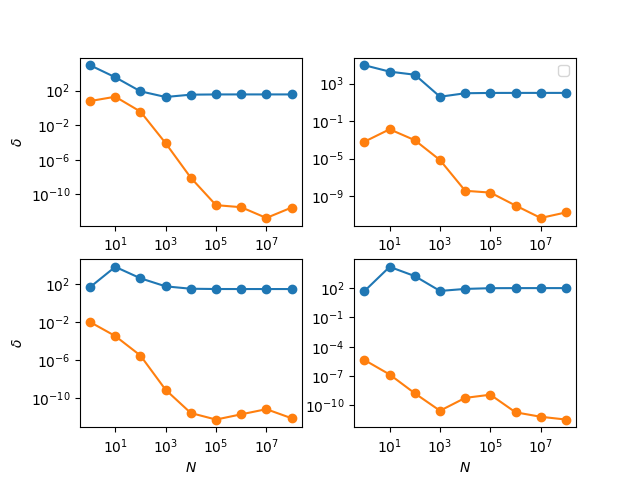
\includegraphics[scale=0.8]{c4/all.png}
  \caption{Relative error of trapezoidal method "$\delta_{Q^T}$" and Filon quadrature "$\delta_{Q^F}$" vs no. of steps $N$ with $a=0,b=100$: (a): $I_1$, $\omega=10$, (b): $I_1$, $\omega=10^3$, (c): $I_2$, $\omega=10$, (d): $I_2$, $\omega=10^3$.}
  \label{figGraphAll}
\end{figure}

The above charts are rendered from numerical data in tables \ref{table1}, \ref{table2}, \ref{table3}, \ref{table4}.  
\vspace{2.5in}


\begin{table}[h!]
    \begin{center}
      \caption{Relative error of trapezoidal method "$\delta_{Q^T}$" and Filon quadrature "$\delta_{Q^F}$" vs no. of steps $N$ on $I_1$ with $a=0,b=100,\omega=10$.}
      \label{table1}
      \pgfplotstabletypeset[
        multicolumn names, % allows to have multicolumn names
        col sep=comma, % the seperator in our .csv file
        display columns/0/.style={
          column name=$N$, % name of first column
          column type={S},string type},  % use siunitx for formatting
        display columns/1/.style={
          column name=$\delta_{Q^T}$,
          column type={S},string type},
        display columns/2/.style={
          column name=$\delta_{Q^F}$,
          column type={S},string type},
        every head row/.style={
          before row={\toprule}, % have a rule at top
          after row={
               & \% & \% \\ % the units seperated by &
              \midrule} % rule under units
              },
          every last row/.style={after row=\bottomrule}, % rule at bottom
      ]{c4/relErrorCosOmega10.csv} % filename/path to file
    \end{center}
  \end{table}


  \begin{table}[h!]
    \begin{center}
      \caption{Relative error of trapezoidal method "$\delta_{Q^T}$" and Filon quadrature "$\delta_{Q^F}$" vs no. of steps $N$ on $I_1$ with $a=0,b=100,\omega=10^3$.}
      \label{table2}
      \pgfplotstabletypeset[
        multicolumn names, % allows to have multicolumn names
        col sep=comma, % the seperator in our .csv file
        display columns/0/.style={
          column name=$N$, % name of first column
          column type={S},string type},  % use siunitx for formatting
        display columns/1/.style={
          column name=$\delta_{Q^T}$,
          column type={S},string type},
        display columns/2/.style={
          column name=$\delta_{Q^F}$,
          column type={S},string type},
        every head row/.style={
          before row={\toprule}, % have a rule at top
          after row={
               & \% & \% \\ % the units seperated by &
              \midrule} % rule under units
              },
          every last row/.style={after row=\bottomrule}, % rule at bottom
      ]{c4/relErrorCosOmega1000.csv} % filename/path to file
    \end{center}
  \end{table}

  \begin{table}[H]
    \begin{center}
      \caption{Relative error of trapezoidal method "$\delta_{Q^T}$" and Filon quadrature "$\delta_{Q^F}$" vs no. of steps $N$ on $I_2$ with $a=0,b=100,\omega=10$.}
      \label{table3}
      \pgfplotstabletypeset[
        multicolumn names, % allows to have multicolumn names
        col sep=comma, % the seperator in our .csv file
        display columns/0/.style={
          column name=$N$, % name of first column
          column type={S},string type},  % use siunitx for formatting
        display columns/1/.style={
          column name=$\delta_{Q^T}$,
          column type={S},string type},
        display columns/2/.style={
          column name=$\delta_{Q^F}$,
          column type={S},string type},
        every head row/.style={
          before row={\toprule}, % have a rule at top
          after row={
               & \% & \% \\ % the units seperated by &
              \midrule} % rule under units
              },
          every last row/.style={after row=\bottomrule}, % rule at bottom
      ]{c4/relErrorPolyOmega10.csv} % filename/path to file
    \end{center}
  \end{table}


  \begin{table}[h!]
    \begin{center}
      \caption{Relative error of trapezoidal method "$\delta_{Q^T}$" and Filon quadrature "$\delta_{Q^F}$" vs no. of steps $N$ on $I_2$ with $a=0,b=100,\omega=10^3$.}
      \label{table4}
      \pgfplotstabletypeset[
        multicolumn names, % allows to have multicolumn names
        col sep=comma, % the seperator in our .csv file
        display columns/0/.style={
          column name=$N$, % name of first column
          column type={S},string type},  % use siunitx for formatting
        display columns/1/.style={
          column name=$\delta_{Q^T}$,
          column type={S},string type},
        display columns/2/.style={
          column name=$\delta_{Q^F}$,
          column type={S},string type},
        every head row/.style={
          before row={\toprule}, % have a rule at top
          after row={
               & \% & \% \\ % the units seperated by &
              \midrule} % rule under units
              },
          every last row/.style={after row=\bottomrule}, % rule at bottom
      ]{c4/relErrorPolyOmega1000.csv} % filename/path to file
    \end{center}
  \end{table}
  \pagebreak

\section{Generalized Filon Method}

The function used in this example is

\begin{equation}
  I_g=\int_a^b dx(x^2+2x^4)e^{i(\omega x+\alpha \sin{\omega_1x})}
\end{equation}

As per the change of variable provided by \eqref{changeOfVariable} and \eqref{changedPhi}, $I'_g$ can be derived as follows


\begin{equation}
  I'_g=\int_{y_{a}}^{y_{b}} dy \frac{x_y^2+2x_y^4}{\omega+\alpha\omega_1cos(\omega_1x(y))}e^{iy}
\end{equation}

There is no analytical solution for $I_g$, therefore the relative error in this example was calculated against
the result obtained from the numerical integration of $I_g$ using
trapezoidal method, at the maximum number of steps $N(10^8)$.\\

The following numerical results were computed using "generalizedFilonQuadrature.cpp" code, found in Annex 1, with the parameters 
$\omega=1.0, \omega_1=2.0, \alpha=0.1, a=0, b=10$.

\begin{figure}[H]
  \centering
  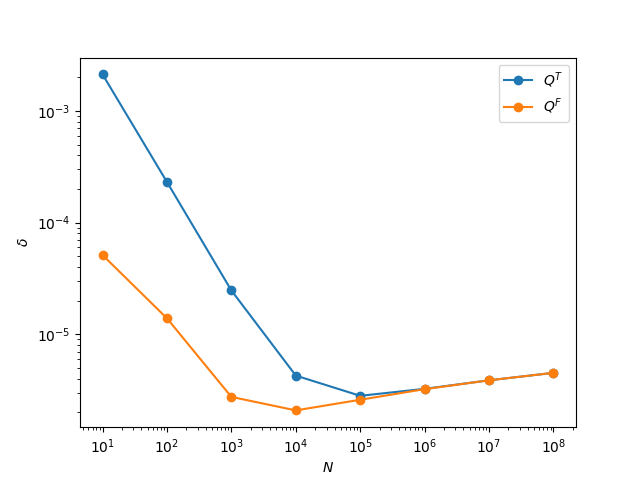
\includegraphics[scale=0.8]{c4/results.png}
  \caption{Relative error of trapezoidal method "$\delta_{Q^T}$" and Filon quadrature "$\delta_{Q^F}$" vs no. of steps $N$,on $I'_g$ against trapezoidal method on $I_g$.}
  \label{figGraphGen}
\end{figure}

The above chart was rendered using the data from \ref{table5}.

\begin{table}[h!]
  \begin{center}
    \caption{Relative error of trapezoidal method "$\delta_{Q^T}$" and Filon quadrature "$\delta_{Q^F}$" vs no. of steps $N$,on $I'_g$ against trapezoidal method on $I_g$.}
    \label{table5}
    \pgfplotstabletypeset[
      multicolumn names, % allows to have multicolumn names
      col sep=comma, % the seperator in our .csv file
      display columns/0/.style={
        column name=$N$, % name of first column
        column type={S},string type},  % use siunitx for formatting
      display columns/1/.style={
        column name=$\delta_{Q^T}$,
        column type={S},string type},
      display columns/2/.style={
        column name=$\delta_{Q^F}$,
        column type={S},string type},
      every head row/.style={
        before row={\toprule}, % have a rule at top
        after row={
             & \% & \% \\ % the units seperated by &
            \midrule} % rule under units
            },
        every last row/.style={after row=\bottomrule}, % rule at bottom
    ]{c4/result.csv} % filename/path to file
  \end{center}
\end{table}


%%% Local Variables:
%%% mode: latex
%%% TeX-master: "../th"
%%% End:

\chapter{Concluzii}









\renewcommand{\contentsname}{References}
\renewcommand\bibname{References} %
\addcontentsline{toc}{chapter}{References}
\markboth{References}{References} %
\bibliographystyle{unsrt}
%
%\bibliographystyle{plain}

\bibliography{Referinte}
\pagebreak


\chapter{Annexes}

\section{filonQuadrature.cpp}

\begin{lstlisting}[language=C++]
const complex<double> iComplex(0,1);
const double pi = acos(-1);


complex<double> filonQuadrature(int n, double a, double b, complex<double> *f(int n , double x[]), double omega){


    double h = (b-a) / (2*n);
    double *x;
    complex<double> *ftab;

    double theta = omega*h;
    double sint = sin(theta), cost = cos(theta);
    double alpha, beta, gamma;

    if ( 6.0 * fabs ( theta ) <= 1.0 ){

        alpha = 2.0 * pow ( theta, 3 )   /   45.0 
              - 2.0 * pow ( theta, 5 )   /  315.0 
              + 2.0 * pow ( theta, 7 )   / 4725.0;
    
        beta  = 2.0                      /     3.0 
              + 2.0 * pow ( theta, 2 )   /    15.0 
              - 4.0 * pow ( theta, 4 )   /   105.0 
              + 2.0 * pow ( theta, 6 )   /   567.0 
              - 4.0 * pow ( theta, 8 )   / 22275.0;

        gamma = 4.0                      /     3.0 
              - 2.0 * pow ( theta, 2 )   /    15.0 
              +       pow ( theta, 4 )   /   210.0 
              -       pow ( theta, 6 )   / 11340.0;
    }
    else{

        alpha = ( pow ( theta, 2 ) + theta * sint * cost 
        - 2.0 * sint * sint ) / pow ( theta, 3 );

        beta = ( 2.0 * theta + 2.0 * theta * cost * cost
        - 4.0 * sint * cost ) / pow ( theta, 3 );

        gamma = 4.0 * ( sint - theta * cost ) / pow ( theta, 3 );
    }

    x = new double [2*n+1];

    for (int j = 0; j <= 2*n; j++)
        x[j] = (double) a + (double) h*j; 

    ftab = f(2*n,x); 
    
    //cout << ftab[1] << endl;

    complex<double> sigma1(0,0);

    for (int j = 0; j<=n; j++)
        sigma1 += ftab[2*j] * exp(iComplex*omega*x[2*j]);

    complex<double> sigma2(0,0);

    for (int j = 1; j<=n; j++)
        sigma2 += ftab[2*j-1] * exp(iComplex*omega*x[2*j-1]);



    complex<double> result = h * (iComplex * alpha * (ftab[0] * exp(iComplex*omega*x[0]) - ftab[2*n] * exp(iComplex*omega*x[2*n])) 
                                   
                                    + beta  * (sigma1 - 0.5 * (ftab[2*n] * exp(iComplex*omega*x[2*n]) + ftab[0] * exp(iComplex*omega*x[0])))
                                   
                                    + gamma  * sigma2

                                  );

    delete [] ftab;
    delete [] x;

    return result;

}

complex<double> trapezoidalMethod(int n, double a, double b, complex<double> *f(int n , double x[]), double omega){
  
      
  double h = (double) (b-a) / n;
  double *x;
  complex<double> *ftab;

 
  x = new double [n+1];

  for (int j = 0; j <= n; j++)
    x[j] = (double) a + (double) h*j; 

  ftab = f(n,x); 

               
  for (int j = 0 ; j < n+1 ; j ++)                              
      ftab[j] *= exp(iComplex*omega*x[j]) ;
    
  complex<double> result = 0;

  for (int j = 1; j < n ; j++)
    result += (double) real(ftab[j])*h;
  
  result += h/2.*(ftab[0]+ftab[n]);

  delete [] ftab;
  delete [] x;

  return result;

}

complex<double> *toIntegratePoly (int n, double x[]){
  
  complex<double> *fx;
  int j;

  fx = new complex<double> [n+1];

  for ( j = 0; j <= n; j++ ){
    fx[j] = x[j] * x[j] + 3*x[j] + pow(x[j],3);
  }

  return fx;
}

complex<double> *toIntegrateCos (int n, double x[]){
  
  complex<double> *fx;
  int j;

  fx = new complex<double> [n+1];

  for ( j = 0; j <= n; j++ ){
    fx[j] = cos(x[j]);
  }

  return fx;
}


\end{lstlisting}

\pagebreak

\section{generalizedFilonQuadrature.cpp}

\begin{lstlisting}
    const complex<double> iComplex(0,1);
const double pi      = acos(-1);
const double omega   = 1;
const double omega1  = 2;
const double A0      = 0.1;
const double phiMax  = 10;
const double phiMin  = 0;



double Aphi(double x){

  return pow(x,2)+2*pow(x,4);

}

complex<double> *complexAphiTab(int n, double x[]){ 

  complex<double> *fx;
  
  fx = new complex<double>[n+1];
  
  for (int i = 0; i <= n; i++){

    fx[i] = (0,0) + Aphi(x[i]);

  }
  return fx;
}




complex<double> hasPhi(double phi){ 
  
  return (0,0) + omega*phi+A0*sin(omega1*phi);
}

complex<double> *hasPhiTab (int n, double phi[]){ 

  complex<double> *fx;

  fx = new complex<double>[n];

  for(int i = 0; i < n; i++)
    fx[i] =  hasPhi(phi[i]) ;

  return fx;

}

double derHasPhi(double x){

  

    return (0,0) + omega + A0*omega1*cos(omega1*x);

}

double interpolate( vector<double> &xData, vector<double> &yData, double x, bool extrapolate )
{
   int size = xData.size();

   int i = 0;                                                                  // find left end of interval for interpolation
   if ( x >= xData[size - 2] )                                                 // special case: beyond right end
   {
      i = size - 2;
   }
   else
   {
      while ( x > xData[i+1] ) i++;
   }
   double xL = xData[i], yL = yData[i], xR = xData[i+1], yR = yData[i+1];      // points on either side (unless beyond ends)
   if ( !extrapolate )                                                         // if beyond ends of array and not extrapolating
   {
      if ( x < xL ) yR = yL;
      if ( x > xR ) yL = yR;
   }

   double dydx = ( yR - yL ) / ( xR - xL );                                    // gradient

   return yL + dydx * ( x - xL );                                              // linear interpolation
}

complex<double> *transVal(int n, double x[]){
  complex<double> *fx;
  
  fx = new complex<double>[n+1];

    double a = phiMin;
    double b = phiMax;
    double h = (double) (b-a)/n; 

   

    double ya=real(hasPhi(a));
    double yb=real(hasPhi(b));
    double yh= (yb-ya)/n;

   vector<double> Yt(n+1), Y(n+1), Xy(n+1), X(n+1);

    
  for (int i = 0 ; i <= n; i ++){
      X.at(i)  = a + i*h; 
      Y.at(i)  = ya + i*yh;
      Yt.at(i) = real(hasPhi(X.at(i)));
      
  }
     
    fx[0]=Aphi(Y.at(0))*exp(iComplex*Y.at(0))/derHasPhi(Y.at(0));
    fx[n]=Aphi(Y.at(n))*exp(iComplex*Y.at(n))/derHasPhi(Y.at(n)); 

  for(int i = 1 ; i < n; i ++){
    double val = Y.at(i); 
    double y = interpolate(X,Yt,val,true); 
    x[i] = y;
    fx[i]=Aphi(y)*exp(iComplex*y)/derHasPhi(y); 
  }

  return fx;
}


complex<double> simpleFilonQuadrature(int n, double a, double b, complex<double> *f(int n , double x[]), double omega){


    double h = (b-a) / (2*n);
    double *x;
    complex<double> *ftab;

    double theta = h;
    double sint = sin(theta), cost = cos(theta);
    double alpha, beta, gamma;
    
    if ( 6.0 * fabs ( theta ) >= 1.0 ){

        alpha = 2.0 * pow ( theta, 3 )   /   45.0 
              - 2.0 * pow ( theta, 5 )   /  315.0 
              + 2.0 * pow ( theta, 7 )   / 4725.0;
    
        beta  = 2.0                      /     3.0 
              + 2.0 * pow ( theta, 2 )   /    15.0 
              - 4.0 * pow ( theta, 4 )   /   105.0 
              + 2.0 * pow ( theta, 6 )   /   567.0 
              - 4.0 * pow ( theta, 8 )   / 22275.0;

        gamma = 4.0                      /     3.0 
              - 2.0 * pow ( theta, 2 )   /    15.0 
              +       pow ( theta, 4 )   /   210.0 
              -       pow ( theta, 6 )   / 11340.0;
    }
    else{
         
        alpha = ( pow ( theta, 2 ) + theta * sint * cost 
        - 2.0 * sint * sint ) / pow ( theta, 3 );

        beta = ( 2.0 * theta + 2.0 * theta * cost * cost
        - 4.0 * sint * cost ) / pow ( theta, 3 );

        gamma = 4.0 * ( sint - theta * cost ) / pow ( theta, 3 );
    }
    
     x = new double [2*n+1];

   
        
    ftab = f(2*n,x); 
    


   

    complex<double> sigma1(0,0);

    for (int i = 0; i<=n; i++)
        sigma1 += ftab[2*i] ;

    complex<double> sigma2(0,0);

    for (int i = 1; i<=n; i++)
        sigma2 += ftab[2*i-1] ;


    complex<double> result = h * (iComplex * alpha * (ftab[0]  - ftab[2*n]) 
                                   
                                    + beta  * (sigma1 - 0.5 * (ftab[2*n]  + ftab[0] ))
                                   
                                    + gamma  * sigma2

                                  );

    delete [] ftab;
    delete [] x;

    return result;

}

complex<double> trapezoidalMethod(int n, double a, double b, complex<double> *f(int n , double x[])){
  
      
  double h = (double) (b-a) / n;
  double *x;
  complex<double> *hasTab;
  complex<double> *ftab;

  hasTab = new complex<double>[n+1];
  x   = new double[n+1]; 

    for (int i = 0; i <= n; i++)
        x[i] = (double) a + (double) h*i; 

    ftab = f(n,x); 
    hasTab = hasPhiTab(n+1,x) ;
               
     for (int i = 0 ; i < n+1 ; i ++){                              
        ftab[i] *= exp(iComplex*hasTab[i]) ;
     }
  complex<double> result(0,0) ;

    for (int i = 1; i < n ; i++)
      result += ftab[i]*h;
  
  result += h/2.*(ftab[0] +ftab[n]);

  delete [] ftab;
  delete [] x;

  return result;

}

complex<double> trapezoidalMethodDebug(int n, double a, double b, complex<double> *f(int n , double x[])){
  
      
  double h = (double) (b-a) / n;
  double *x;
  complex<double> *ftab;

  x   = new double[n+1]; 

    for (int i = 0; i <= n; i++)
        x[i] = (double) a + (double) h*i; 

    ftab = f(n,x); 


  complex<double> result(0,0) ;

    for (int i = 1; i < n ; i++)
      result += ftab[i]*h;
  
  result += h/2.*(ftab[0] +ftab[n]);

  delete [] ftab;
  delete [] x;

  return result;

}

\end{lstlisting}

\end{document}





